\documentclass[12pt, a4paper]{article}

\usepackage[utf8]{inputenc}
\usepackage[T1]{fontenc}
\usepackage[russian]{babel}
\usepackage[oglav,spisok,boldsect, figwhole]{./style/fn2kursstyle1}
\graphicspath{{./style/}{./figures/}}
%\usepackage{float}%"Плавающие" картинки
\usepackage{multirow}
\usepackage{subcaption}
\usepackage{float}%"Плавающие" картинки
%Римские цифры
\newcommand{\RomanNumeralCaps}[1]
{\MakeUppercase{\romannumeral #1}}

\usepackage{enumitem} 
\usepackage{amsmath}
\usepackage{comment}
\usepackage{makecell}

%Параметры титульника
\title{Численное решение краевых задач для одномерного волнового уравнения}
\group{ФН2-62Б}
\author{З.И.~Абрамов, Г.А.~Швецов}
\supervisor{С.А.~Конев}
\date{2023}
\begin{document}
	\newcommand{\pl}{\partial}
	\maketitle
	
	\tableofcontents
	
	\newpage
	
	\section{Контрольные вопросы}
	% TODO %%%%%%%%%%%%%%%%%%%%%%%%%%%%%%%%%%%%%%%%%%%%%%%%%%%%
	\begin{enumerate}
		\item \textit{Предложите разностные схемы, отличные от схемы «крест», для численного решения задачи (3.1)–(3.4).}
		\smallskip
		
		Для решения волнового уравнения можно построить следующие разностные схемы:
		\begin{enumerate}
			\item явную схему вида
			\[
			\frac{y_i^{j+1} - 2y_i^j + y_i^{j-1}}{\tau^2} = c^2 \frac{y_{i+1}^{j-1} -2 y_i^{j-1} + y_{i-1}^{j-1}}{h^2},			
			\]
			однако она является абсолютно неустойчивой;
			\item неявную схему вида
			\[
			\frac{y_i^{j+1} - 2y_i^j + y_i^{j-1}}{\tau^2} = c^2 \frac{y_{i+1}^{j+1} -2 y_i^{j+1} + y_{i-1}^{j+1}}{h^2};
			\]
			Проверим ее на устойчивость \textit{методом гармоник}.
			
			Введем замену $y_i^j=\rho^je^{\tilde i i \varphi}$. Тогда
			\begin{multline*}
\dfrac1{\tau^2}\left(\rho^{j+1}e^{\tilde i i \varphi} - 2\rho^je^{\tilde i i \varphi} + \rho^{j-1}e^{\tilde i i \varphi}\right) =\\= \dfrac{c^2}{h^2} \left(\rho^{j+1}e^{\tilde i (i+1) \varphi} -2 \rho^{j+1}e^{\tilde i i \varphi} + \rho^{j+1}e^{\tilde i (i-1) \varphi}\right),
\end{multline*}
\begin{multline*}
\rho^{j+1}e^{\tilde i i \varphi} - 2\rho^je^{\tilde i i \varphi} + \rho^{j-1}e^{\tilde i i \varphi} =\\= \dfrac{c^2\tau^2}{h^2} \left(\rho^{j+1}e^{\tilde i (i+1) \varphi} -2 \rho^{j+1}e^{\tilde i i \varphi} + \rho^{j+1}e^{\tilde i (i-1) \varphi}\right)\left.\right|:\rho^{j},\;:e^{\tilde i i \varphi},
\end{multline*}
\begin{eqnarray*}
	\centering
	&\rho-2+\rho^{-1}=\dfrac{c^2\tau^2}{h^2}\left(2\rho\cos\varphi-2\rho\right),\\
	&\rho-2+\rho^{-1}=-4\rho\dfrac{c^2\tau^2}{h^2}\sin^2\frac{\varphi}{2},\\
	&\left(1+4\dfrac{c^2\tau^2}{h^2}\sin^2\frac{\varphi}{2}\right)\rho^2-2\rho+1=0,\\
	& D = -16\dfrac{c^2\tau^2}{h^2}\sin^2\frac{\varphi}{2}<0,\\
&\rho_1 = \dfrac{1-2\tilde i \sfrac{c\tau}{h}\sin \frac{\varphi}{2}}{1+4\sfrac{c^2 \tau^2}{h^2}\sin^2 \frac{\varphi}{2}},\quad \rho_2 = \dfrac{1+2\tilde i \sfrac{c\tau}{h}\sin \frac{\varphi}{2}}{1+4\sfrac{c^2 \tau^2}{h^2}\sin^2 \frac{\varphi}{2}},\\
&|\rho_{1,2}| = \dfrac{1}{1+4\sfrac{c^2 \tau^2}{h^2}\sin^2 \frac{\varphi}{2}}\sqrt{1+4\sfrac{c^2\tau^2}{h^2}\sin^2\sfrac{\varphi}{2}},\\
&|\rho_{1,2}| = \dfrac{1}{\sqrt{1+4\sfrac{c^2 \tau^2}{h^2}\sin^2 \frac{\varphi}{2}}}\le1,
\end{eqnarray*}	
следовательно, неявная схема устойчива.
			\item неявную схему вида
			\[
			\frac{y_i^{j+1} - 2y_i^j + y_i^{j-1}}{\tau^2} = c^2 \frac{(y_{i+1}^{j-1} -2 y_i^{j-1} + y_{i-1}^{j-1}) + (y_{i+1}^{j+1} -2 y_i^{j+1} + y_{i-1}^{j+1})}{2 h^2},
			\]
			Проверим ее на устойчивость \textit{методом гармоник}.
			
			Введем замену $y_i^j=\rho^je^{\tilde i i \varphi}$. Тогда
			\begin{multline*}
				\dfrac1{\tau^2}\left(\rho^{j+1}e^{\tilde i i \varphi} - 2\rho^je^{\tilde i i \varphi} + \rho^{j-1}e^{\tilde i i \varphi}\right) =\\= \dfrac{c^2}{2h^2} \left(\left(\rho^{j-1}e^{\tilde i (i+1) \varphi} -2 \rho^{j-1}e^{\tilde i i \varphi} + \rho^{j-1}e^{\tilde i (i-1) \varphi}\right)\right.+\\+\left.\left(\rho^{j+1}e^{\tilde i (i+1) \varphi} -2 \rho^{j+1}e^{\tilde i i \varphi} + \rho^{j+1}e^{\tilde i (i-1) \varphi}\right)\right)\left.\right|:\rho^{j},\;:e^{\tilde i i \varphi},
			\end{multline*}
			\begin{eqnarray*}
				\centering
				&\rho-2+\rho^{-1}=\dfrac{c^2\tau^2}{2h^2}\left(2\rho^{-1}\cos\varphi-2\rho^{-1}+2\rho\cos\varphi-2\rho\right),\\
				&\rho-2+\rho^{-1}=\dfrac{c^2\tau^2}{2h^2}\left(-4\rho^{-1}\sin^2\frac{\varphi}{2}-4\rho\sin^2\frac{\varphi}{2}\right),\\
				&\rho-2+\rho^{-1}=-2\dfrac{c^2\tau^2}{h^2}\sin^2\frac{\varphi}{2}\left(\rho^{-1}+\rho\right),\\
				&\left(1+2\dfrac{c^2\tau^2}{h^2}\sin^2\frac{\varphi}{2}\right)\rho^2-2\rho+\left(1+2\dfrac{c^2\tau^2}{h^2}\sin^2\frac{\varphi}{2}\right)=0,\\
				& D = -16\dfrac{c^2\tau^2}{h^2}\sin^2\frac{\varphi}{2}\left(1+\dfrac{c^2\tau^2}{h^2}\sin^2\frac{\varphi}{2}\right)<0,\\
				&\rho_{1,2} = \dfrac{1\pm2\tilde i \sfrac{c\tau}{h}\sin \frac{\varphi}{2}\sqrt{1+\sfrac{c^2\tau^2}{h^2}\sin^2\frac{\varphi}{2}}}{1+2\sfrac{c^2 \tau^2}{h^2}\sin^2 \frac{\varphi}{2}},\\
				&|\rho_{1,2}| = 1,
			\end{eqnarray*}	
			следовательно, неявная схема является абсолютно устойчивой.
	\end{enumerate}
		\item \textit{Постройте разностную схему с весами для уравнения колебаний струны.\\ Является ли такая схема устойчивой и монотонной?}
		\smallskip
		
		Построим неявную схему с весами:
	\[
	\frac{\hat y-2y+\check y}{\tau^2}=\Lambda\left(\sigma\hat y+(1-2\sigma)y+\sigma \check y\right),\quad \Lambda y= \frac{c^2}{h^2}(y_{+1}-2y+y_{-1}).
	\]
	Погрешность аппроксимации $\psi=O(\tau^2+h^2)$ $\forall\sigma\in[0,1]$.
	
	Используя, например, энергетический метод можно получить условие устойчивости\cite{galanin}:
	\[
	\sigma \ge \frac14 - \frac{h^2}{4 c^2 \tau^2}.
	\]
	
	Такой же результат можно получить и методом гармоник. Подставим в схему $y_i^j = \rho^j e^{\tilde i i \varphi}$, поделив левую и правую части $\rho^{j-1} e^{\tilde i i \varphi}$ и вынеся за скобку в правой части $e^{\tilde i \varphi} -2 + e^{-\tilde i \varphi}$:
	\[
	\dfrac{\rho^2 -2\rho + 1}{\tau^2} = \dfrac{c^2}{h^2}(e^{\tilde i \varphi} -2 + e^{-\tilde i \varphi}) (\sigma \rho^2 + (1-2\sigma)\rho+\sigma).
	\]
	Вынесенный множитель можно записать как $-4\sin^2\sfrac\varphi2$. Тогда после замены и домножения на $\tau^2$ получаем следующее выражение:
	\begin{eqnarray*}
		&\rho^2 -2\rho + 1 = -4 \left(\dfrac{c \tau}{h}\right)^2 \sin^2\sfrac\varphi2 (\sigma \rho^2 + (1-2\sigma)\rho+\sigma),\\
		& \left(1+4\sigma\left(\dfrac{c \tau}{h}\right)^2 \sin^2\sfrac\varphi2\right)\rho^2 + \left(4 \left(\dfrac{c \tau}{h}\right)^2 \sin^2\sfrac\varphi2(1-2\sigma) - 2\right) \rho + \left(1+4\sigma\left(\dfrac{c \tau}{h}\right)^2 \sin^2\sfrac\varphi2\right) = 0,\\
		& \rho^2 - 2\dfrac{1- 2 \left(\dfrac{c \tau}{h}\right)^2 \sin^2\sfrac\varphi2(1-2\sigma)}{1+4\sigma\left(\sfrac{c \tau}{h}\right)^2 \sin^2\sfrac\varphi2}\rho + 1 =0.
	\end{eqnarray*}
	
	По теореме Виета произведение корней $\rho_1 \rho_2 = 1$. Значит, условие устойчивости $\rho \le 1$ может быть выполнено, если $|\rho_1|=|\rho_2|=1$. Для уравнения с действительными коэффициентами это возможно, если корни являются комплексно сопряженными, т.е. дискриминант не должен быть положительным:
	\begin{eqnarray*}
		&D/4 = \left(\dfrac{1- 2 \left(\dfrac{c \tau}{h}\right)^2 \sin^2\sfrac\varphi2(1-2\sigma)}{1+4\sigma\left(\sfrac{c \tau}{h}\right)^2 \sin^2\sfrac\varphi2}\right)^2 - 1 \le 0,\\
		&\left|\dfrac{1- 2 \left(\sfrac{c \tau}{h}\right)^2 \sin^2\sfrac\varphi2(1-2\sigma)}{1+4\sigma\left(\sfrac{c \tau}{h}\right)^2 \sin^2\sfrac\varphi2}\right| \le 1,\\
		&\left|1- 2 \left(\sfrac{c \tau}{h}\right)^2 \sin^2\sfrac\varphi2(1-2\sigma)\right| \le \left|1+4\sigma\left(\sfrac{c \tau}{h}\right)^2 \sin^2\sfrac\varphi2\right| = 1+4\sigma\left(\sfrac{c \tau}{h}\right)^2 \sin^2\sfrac\varphi2, \\
		& -1 -4\sigma\left(\sfrac{c \tau}{h}\right)^2 \sin^2\sfrac\varphi2 \le 1- 2 \left(\sfrac{c \tau}{h}\right)^2 \sin^2\sfrac\varphi2(1-2\sigma) \le 1 +4\sigma\left(\sfrac{c \tau}{h}\right)^2 \sin^2\sfrac\varphi2,\\
		& -1 - 8\sigma\left(\sfrac{c \tau}{h}\right)^2 \sin^2\sfrac\varphi2 \le 1- 2 \left(\sfrac{c \tau}{h}\right)^2 \sin^2\sfrac\varphi2 \le 1. 
	\end{eqnarray*}
	
	В полученном выражении правое неравенство выполняется автоматически. Рассмотрим левое:
	\begin{eqnarray*}
		& 2- 2(1-4\sigma) \left(\sfrac{c \tau}{h}\right)^2 \sin^2\sfrac\varphi2 \ge 0, \quad 1-(1-4\sigma) \left(\sfrac{c \tau}{h}\right)^2 \sin^2\sfrac\varphi2 \ge 0,\\
		& 1 - 4\sigma \le \dfrac{h^2}{c^2 \tau^2 \sin^2\sfrac\varphi2}, \quad \sigma \ge \dfrac14 - \dfrac{h^2}{4 c^2 \tau^2 \sin^2\sfrac\varphi2}.
	\end{eqnarray*}
	
	Данное неравенство должно выполняться при любом значении $\varphi$. Учитывая этот факт, получаем итоговое выражение:
	\[
	\sigma \ge \dfrac14 - \dfrac{h^2}{4 c^2 \tau^2}.
	\]
	
	При $\sigma\ge\sfrac14$ схема безусловно устойчива. Если $\sigma<\sfrac14$, то схема условно устойчива при $c\tau\le \sfrac{h}{\sqrt{1-4\sigma}}$. Схема при $\sigma=0$ переходит в схему <<крест>>, а условие устойчивости --- в условие Куранта.
	
	Проверим данную схему на монотонность. Распишем ее:
	\begin{multline*}
		\frac{y_i^{j+1}-2y_i^j+y_i^{j-1}}{\tau^2} = \frac{c^2}{h^2} \Big(\sigma(y_{i+1}^{j+1}-2y_i^{j+1}+y_{i-1}^{j+1}) + \\
		%
		+ (1-2\sigma)(y_{i+1}^j-2y_i^j+y_{i-1}^j) + \sigma(y_{i+1}^{j-1}-2y_i^{j-1}+y_{i-1}^{j-1})\Big).
	\end{multline*}
	
	Теперь приведем к каноническому виду, т.е. оставим слева только $y_i^{j+1}$:
	\begin{multline*}
		\left(\frac1{\tau^2} + 2\frac{c^2\sigma}{h^2}\right) y_i^{j+1} = \frac{c^2\sigma}{h^2} y_{i+1}^{j+1} + \frac{c^2\sigma}{h^2} y_{i-1}^{j+1} + \frac{c^2(1-2\sigma)}{h^2}y_{i+1}^j + \left(-2 \frac{c^2(1-2\sigma)}{h^2} + \frac2{\tau^2}\right)y_i^j + \\ + \frac{c^2(1-2\sigma)}{h^2}y_{i-1}^j + \frac{c^2\sigma}{h^2} y_{i+1}^{j-1} + \left(-2\frac{c^2\sigma}{h^2} - \frac1{\tau^2}\right)y_i^{j-1} + \frac{c^2\sigma}{h^2} y_{i-1}^{j-1}.
	\end{multline*}
	
	Из-за наличия отрицательного коэффициента у переменной $y_i^{j-1}$ условие положительности коэффициентов не выполняется.
		
		\item \textit{Предложите способ контроля точности полученного решения.}
		\smallskip
		
		Пусть численная схема имеет $p$-й порядок сходимости по пространству и $q$-й по времени, т.е. верно следующее выражение:
		\[
		u(x_i, t_j) = y_i^j + O(h^p + \tau^q).
		\]
		
		Теперь распишем $O(h^p + \tau^q)$ более подробно:
		\[
		u(x_i, t_j) = y_i^j + C_x(x, t) h^p + C_t(x, t) \tau^q + O(h^{p+1} + \tau^{q+1}),
		\]
		где $C_x$ и $C_t$ --- некоторые непрерывные функции, которые в общем случае являются вектор-функциями (если $u$ --- вектор-функция). В дальнейшем для простоты будем опускать их аргументы.
		
		Далее сгущаем сетку в $r_x$ раз по пространству и в $r_t$ раз по времени. Тогда получаем, что
		\[
		u(x_{r_x i}, t_{r_t j}) = y_{r_x i}^{r_t j} + C_x \left(\frac{h}{r_x}\right)^p + C_t \left(\frac{\tau}{r_t}\right)^q + O\left(\left(\frac{h}{r_x}\right)^{p+1} + \left(\frac{\tau}{r_t}\right)^{q+1}\right),
		\]
		где под $(r_x i, r_t j)$ понимается номер узла сгущенной сетки, координаты которого совпадают с координатами узла, имеющего номер $(i, j)$, исходной сетки. Таким образом, $u(x_{r_x i}, t_{r_t j}) = u(x_i, t_j)$. Однако это неверно для $y_{r_x i}^{r_t j}$ и $y_i^j$.
		
		Для того, чтобы теперь получить оценку погрешности, потребуем выполнения $r_x^p = r_t^q$. Данное условие называется условием согласования коэффициентов сгущения по времени и пространству.
		
		Введем следующее обозначение, описывающее искомую оценку погрешности на сгущенной сетке:
		\[
		R(x, t) =  C_x \left(\frac{h}{r_x}\right)^p + C_t \left(\frac{\tau}{r_t}\right)^q.
		\]
		
		Приходим к системе, через которую можно выразить $R$ путем вычитания одной строки из другой:
		\[
		\begin{cases}
			u(x_i, t_j) = y_i^j + r_x^p R + O(h^{p+1} + \tau^{q+1}),\\
			u(x_i, t_j) = y_{r_x i}^{r_t j} + R + O(h^{p+1} + \tau^{q+1})
		\end{cases} \Rightarrow y_{r_x i}^{r_t j} - y_i^j \approx (r_x^p - 1) R \Rightarrow R \approx \frac{y_{r_x i}^{r_t j} - y_i^j}{r_x^p - 1}.
		\]
		
		Таким образом, если для некоторой заданной точности $\varepsilon$ получили, что $R \ge \varepsilon$, то следует дробить сетку до тех пор пока данное выражение не станет ложным. В качестве итогового ответа можно взять решение на последней сетке.
		% TODO
		
		\item \textit{Приведите пример трехслойной схемы для уравнения теплопроводности. Как реализовать вычисления по такой разностной схеме? Является ли эта схема устойчивой?}
		\smallskip
		
		В качестве трехслойной схемы для уравнения теплопроводности можно привести схему Ричардсона:
		\[
		\frac{\hat y - \check y}{2\tau}=K\frac{y_{+1}-2y+y_{-1}}{h^2}
		\]
		Погрешность аппроксимации $\psi=O(\tau^2+h^2)$.
		
		Схема является явной, однако требует задания двух начальных временных слоев. Значение на втором временном слое можно получить из первого, заданного начальным условием, следующим образом:
		\[
		y_i^1 \approx u(\tau, x_i) = u(0, x_i) + \tau u_t(0, x_i) + O(\tau^2), \quad i = \overline{1, N-1}.
		\]
		
		Значения $y_0^1$ и $y_N^1$ определяются из граничных условий (при условии, что они являются условиями I рода). Заметим, что первое слагаемое можно найти используя начальное условие $u(0, x) = \varphi(x)$, а из самого уравнения теплопроводности известно, что $u_t = K u_{xx}$, т.е. $u_t(0, x_i) = K u_{xx}(0, x_i) = K \varphi''(x_i)$. Заменяя вторую производную функции $\varphi$ на ее разностный аналог (при этом второй порядок аппроксимации остается), получаем итоговую формулу:
		\[
		y_i^1 = \varphi(x_i) + \tau \varphi_{\bar{x}x}(x_i), \quad i = \overline{1, N-1}.
		\]
		
		Исследуем схему на устойчивость \textit{методом гармоник:}
		\[
		\frac{\hat y - \check y}{2\tau}=K\frac{y_{+1}-2y+y_{-1}}{h^2}\qquad \Rightarrow \qquad \hat y = \frac{2 K\tau}{h^2}(y_{+1}-2y+y_{-1}) + \check y.
		\]
		
		Введем замену $y_i^j=\rho^je^{\tilde i i \varphi}$. Тогда
		\begin{eqnarray*}
			& \rho^{j+1}e^{\tilde i i \varphi} = \dfrac{2 K\tau}{h^2}(\rho^je^{\tilde i (i+1) \varphi}-2\rho^je^{\tilde i i \varphi}+\rho^je^{\tilde i (i-1) \varphi}) + \rho^{j-1}e^{\tilde i i \varphi} \left.\right|:\rho^{j},\;:e^{\tilde i i \varphi},\\
			& \rho=\dfrac{2K\tau}{h^2}(e^{\tilde i \varphi}-2+e^{-\tilde i \varphi})+\rho^{-1}, \\
			& \rho=-\dfrac{8K\tau}{h^2}\sin^2\dfrac{\varphi}{2}+\rho^{-1},\\
			& \rho^2+\dfrac{8K\tau}{h^2}\sin^2\dfrac{\varphi}{2}\rho-1=0.
		\end{eqnarray*}
		
		Видно, что его дискриминант
		\[
		D/4 = \left(\frac{4K\tau}{h^2} \sin^2 \frac\varphi2\right)^2 + 1 > 0,
		\]
		следовательно, корни действительны и различны, причем $\rho_1 \rho_2 = -1$. Отсюда получаем, что один из корней заведомо больше единицы по модулю. Таким образом схема является безусловно неустойчивой.
		
		\begin{comment}
			\[
			\rho_{1,2}=-\frac{4K\tau}{h^2}\sin^2\frac{\varphi}{2} \pm \sqrt{\frac{16K^2\tau^2}{h^4}\sin^4\frac{\varphi}{2}+1}
			\]
			Проверим условие устойчивости $|\rho|\le1$
			\begin{gather*}
				\left|-\frac{4K\tau}{h^2}\sin^2\frac{\varphi}{2} \pm \sqrt{\frac{16K^2\tau^2}{h^4}\sin^4\frac{\varphi}{2}+1}\right|\le\left|-\frac{4K\tau}{h^2}\sin^2\frac{\varphi}{2}\right|+\left|\sqrt{\frac{16K^2\tau^2}{h^4}\sin^4\frac{\varphi}{2}+1}\right|\le\\\le\frac{4K\tau}{h^2}+\sqrt{\left(\frac{4K\tau}{h^2}\right)^2+1}\ge 1.
			\end{gather*}
			Данная схема по методу гармоник оказалась неустойчивой.
			%Получилось почему-то неустойчивое, с Лукиным номер делали этот
		\end{comment}
	\end{enumerate}
	\newpage
	\section{Результаты}
	\paragraph{Тестовая задача 1}
	\[
	u_{tt}=u_{xx},\;0<x<1,\;t>0,
	\]
	\[
	u(x,0)=\sin{\pi x},\; u_t(x,0)=0,\;0<x<1,
	\]
	\[
	u(0,t)=0,\;u(1,t)=0,\;t>0.
	\]
	Точное решение:
	\[
u(x,t)=\sin{\pi x} \cos{\pi t}.
	\]
	Численное решение ($\tau = 0.01,\;h=0.02,\;T=10.0,\;L=1.0$):	
		\begin{figure}[H]
		\centering
		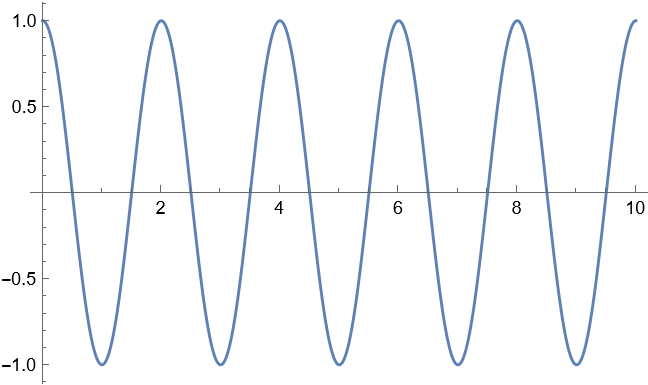
\includegraphics[width=0.7\linewidth]{test1numerical}
		\caption{Численное решение}
	\end{figure}
	График погрешности:
		\begin{figure}[H]
		\centering
		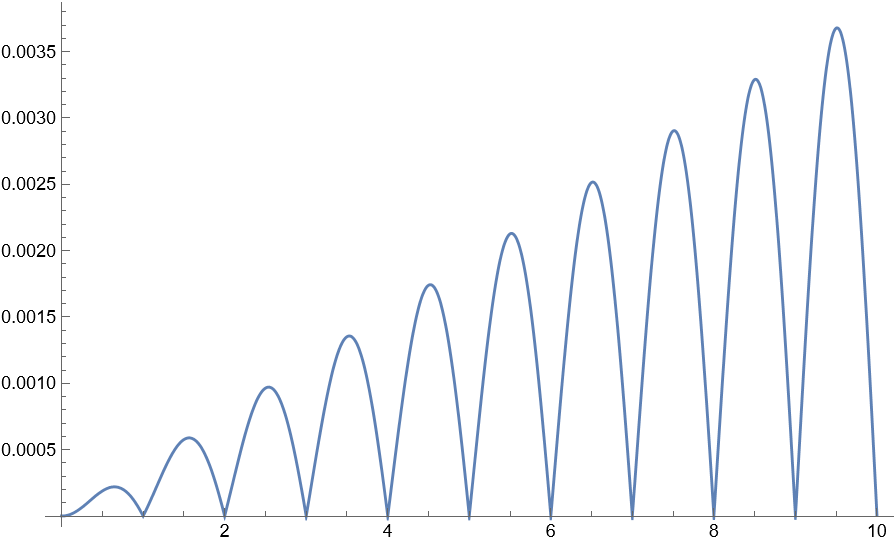
\includegraphics[width=0.7\linewidth]{test1pogr}
		\caption{Разность численного и точного решения}
	\end{figure}

	\paragraph{Тестовая задача 2}
\[
u_{tt}=u_{xx},\;0<x<1,\;t>0,
\]
\[
u(x,0)=x(1-x),\; u_t(x,0)=0,\;0<x<1,
\]
\[
u(0,t)=0,\;u(1,t)=0,\;t>0.
\]
Точное решение:
\[
u(x,t)=\frac{8}{\pi^3}\sum\limits_{n=0}^{\infty}\frac{1}{(2n+1)^3}\sin{()2n+1)\pi x}\cos{(2n+1)\pi t}.
\]
Численное решение ($\tau = 0.01,\;h=0.02,\;T=10.0,\;L=1.0,\;k=10$):	
\begin{figure}[H]
	\centering
	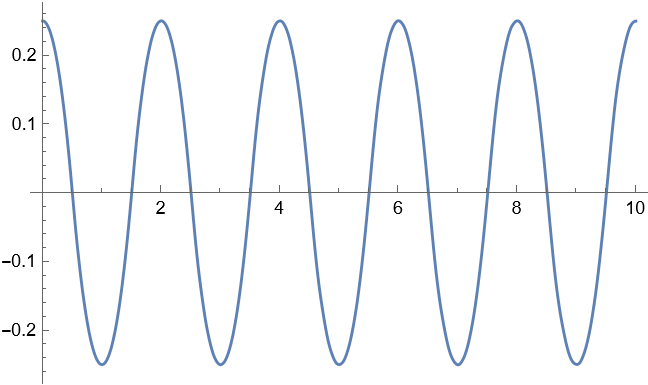
\includegraphics[width=0.7\linewidth]{test2numerical}
	\caption{Численное решение}
\end{figure}
График погрешности:
\begin{figure}[H]
	\centering
	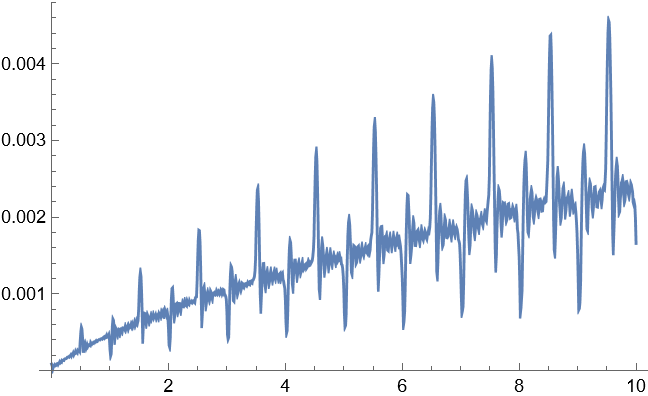
\includegraphics[width=0.7\linewidth]{test2pogr}
	\caption{Разность численного и точного решения}
\end{figure}

	\paragraph{Тестовая задача 3}
\[
u_{tt}=u_{xx},\;-2<x<2,\;t>0,
\]
\[
u(-2,t)=0,\;u(2,t)=0,\;t>0,
\]
\[
u(x,0)=f(x),\; u_t(x,0)=0,\;-2<x<2,
\]
\[
f(x)=
\begin{cases}
	1,\;x\in[-\frac13,\frac13],\\
	0,\;x\notin[-\frac13,\frac13].
\end{cases}
\]
\begin{enumerate}
\item $\gamma =0.1\,(\tau = 0.01 ,h =0.1)$:
\begin{figure}[H]
	\centering
	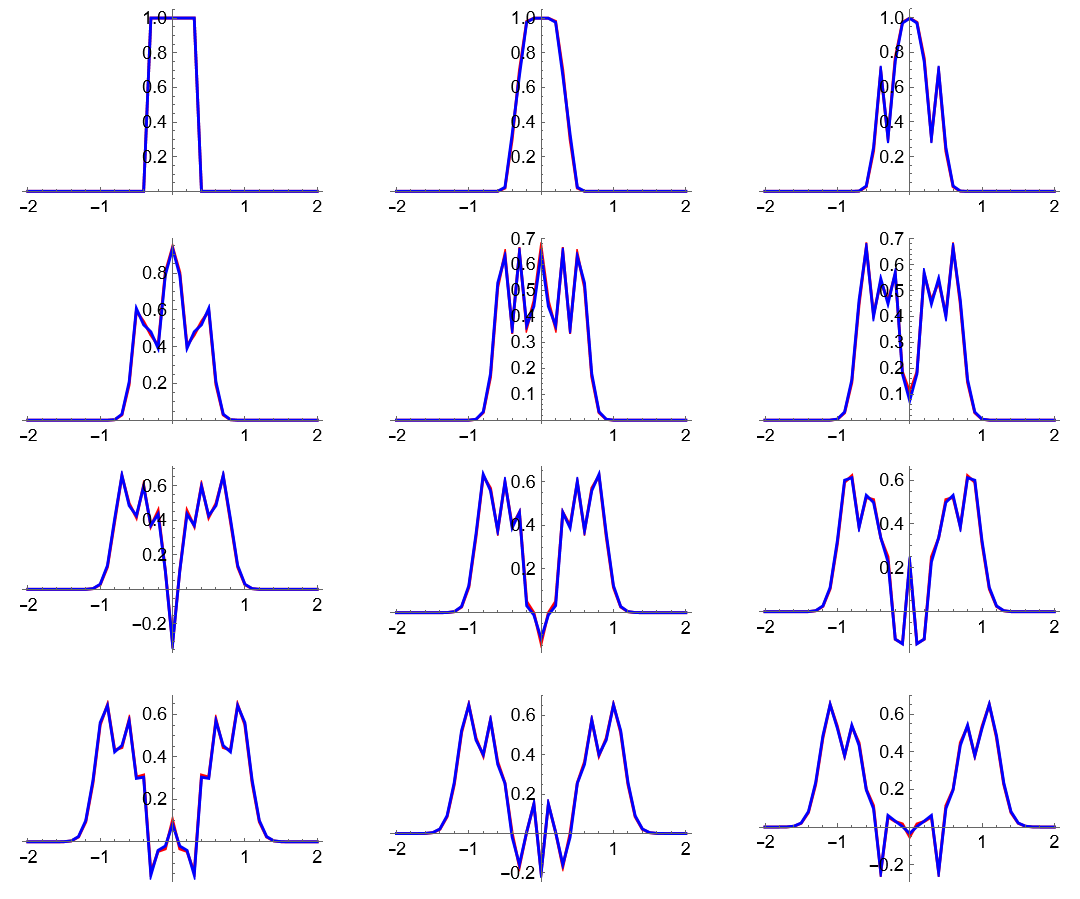
\includegraphics[width=0.7\linewidth]{task1_0.1}
	\caption{Численное решение}
\end{figure}
\newpage
\item $\gamma =0.5\,(\tau = 0.01 ,h =0.02)$:
\begin{figure}[H]
	\centering
	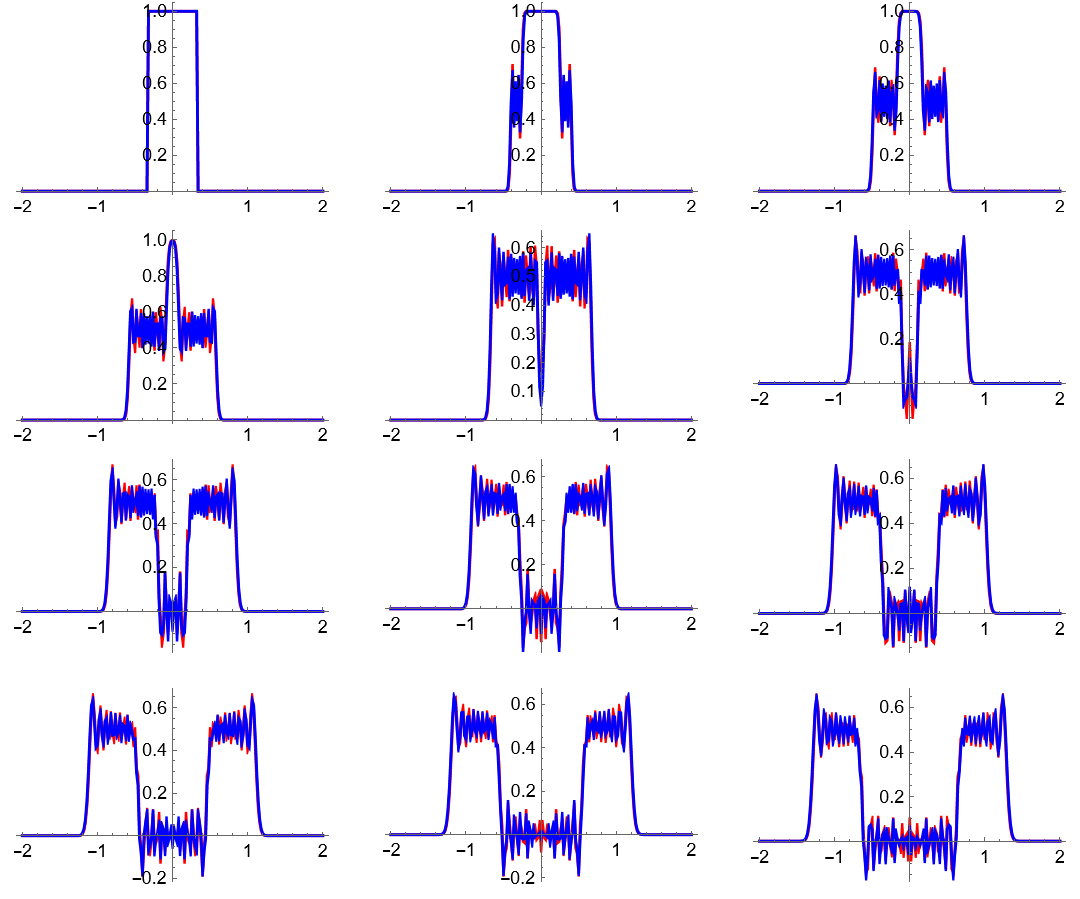
\includegraphics[width=0.7\linewidth]{task1_0.5}
	\caption{Численное решение}
\end{figure}
\item $\gamma =0.75\,(\tau = 0.1125 ,h =0.15)$:
\begin{figure}[H]
	\centering
	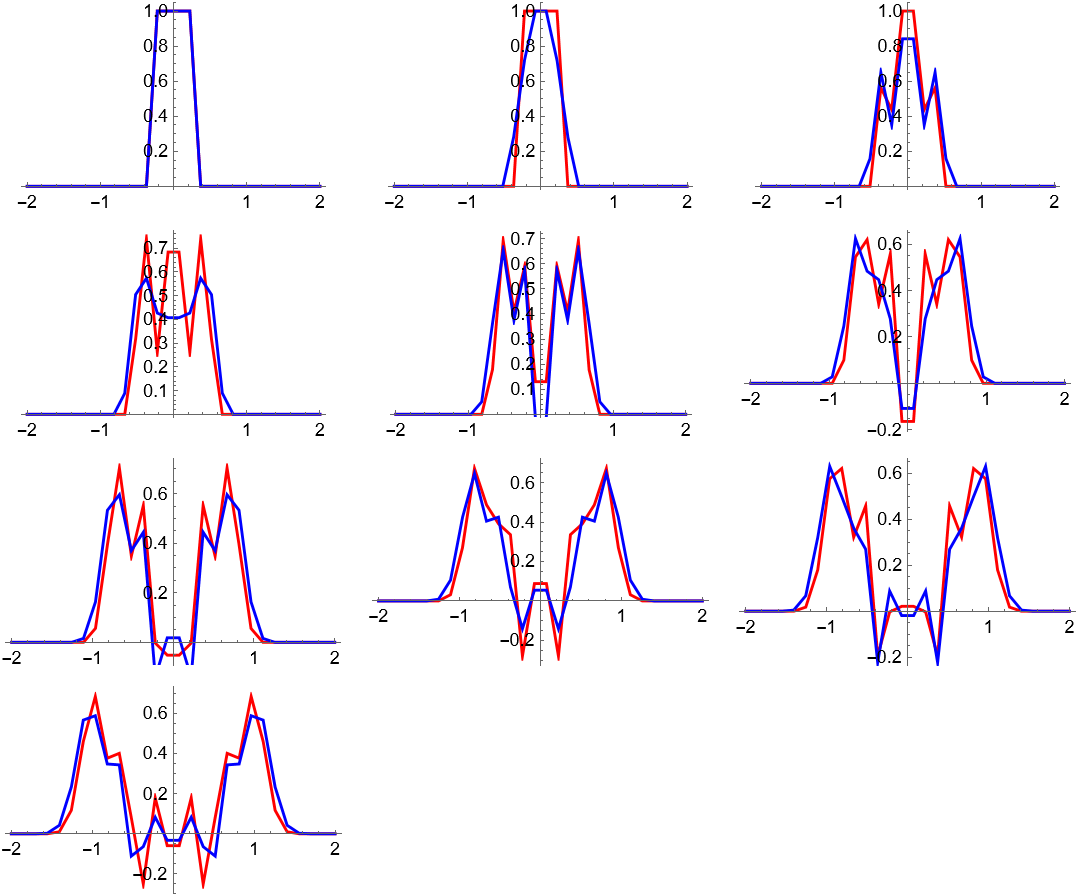
\includegraphics[width=0.7\linewidth]{task1_0.75}
	\caption{Численное решение}
\end{figure}
\newpage
\item $\gamma =1.0\,(\tau = 0.01 ,h =0.01)$:
\begin{figure}[H]
	\centering
	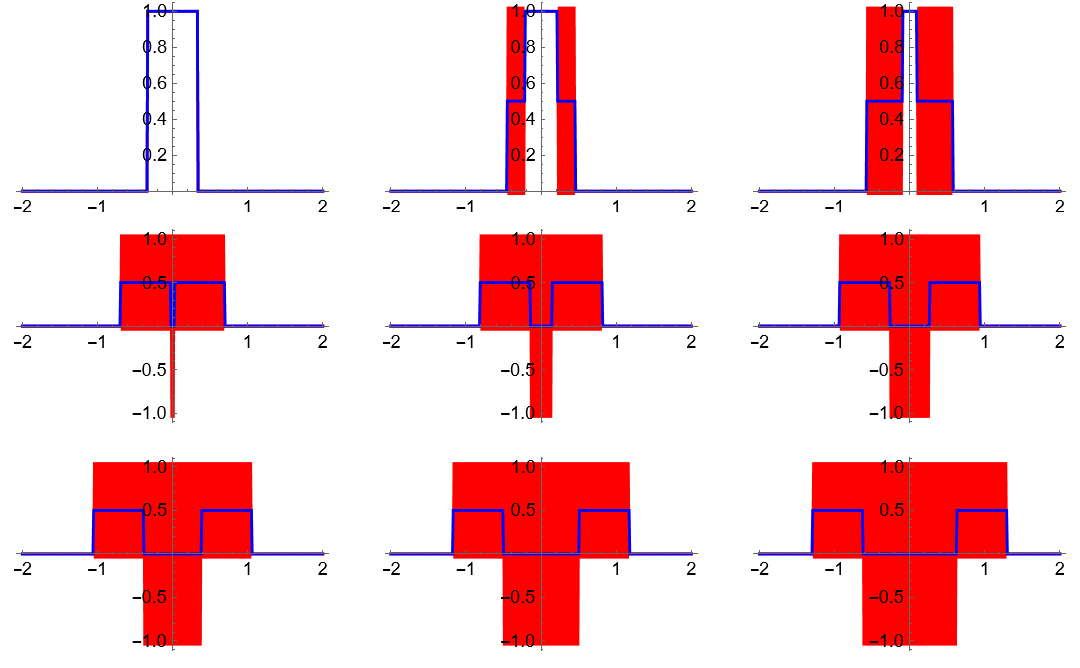
\includegraphics[width=0.7\linewidth]{task1_1.0}
	\caption{Численное решение}
\end{figure}
\end{enumerate}
	\paragraph{Тестовая задача 4}
\[
u_{tt}=u_{xx},\;-1<x<1,\;t>0,
\]
\[
u(-1,t)=0,\;u(1,t)=0,\;t>0.
\]
\[
u(x,0)=0,\; u_t(x,0)=g(x),\;-1<x<1,
\]
\[
g(x)=
\begin{cases}
	1-2|x|,\;x\in[-\frac12,\frac12],\\
	0,\;x\notin[-\frac12,\frac12].
\end{cases}
\]
Численное решение
\begin{enumerate}
	\item $\gamma =0.1\,(\tau = 0.01 ,h =0.1)$:
	\begin{figure}[H]
		\centering
		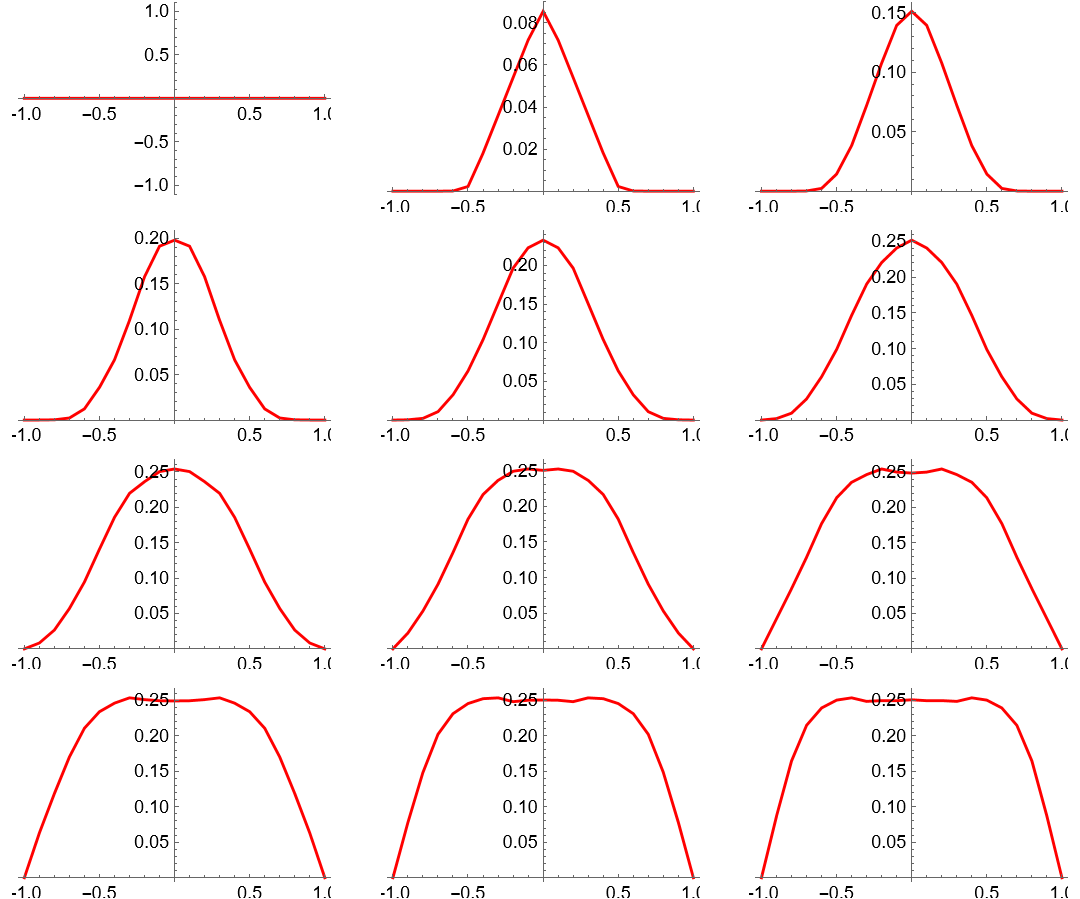
\includegraphics[width=0.5\linewidth]{task2_0.1}
		\caption{Численное решение}
	\end{figure}
	\item $\gamma =0.5\,(\tau = 0.01 ,h =0.02)$:
	\begin{figure}[H]
		\centering
		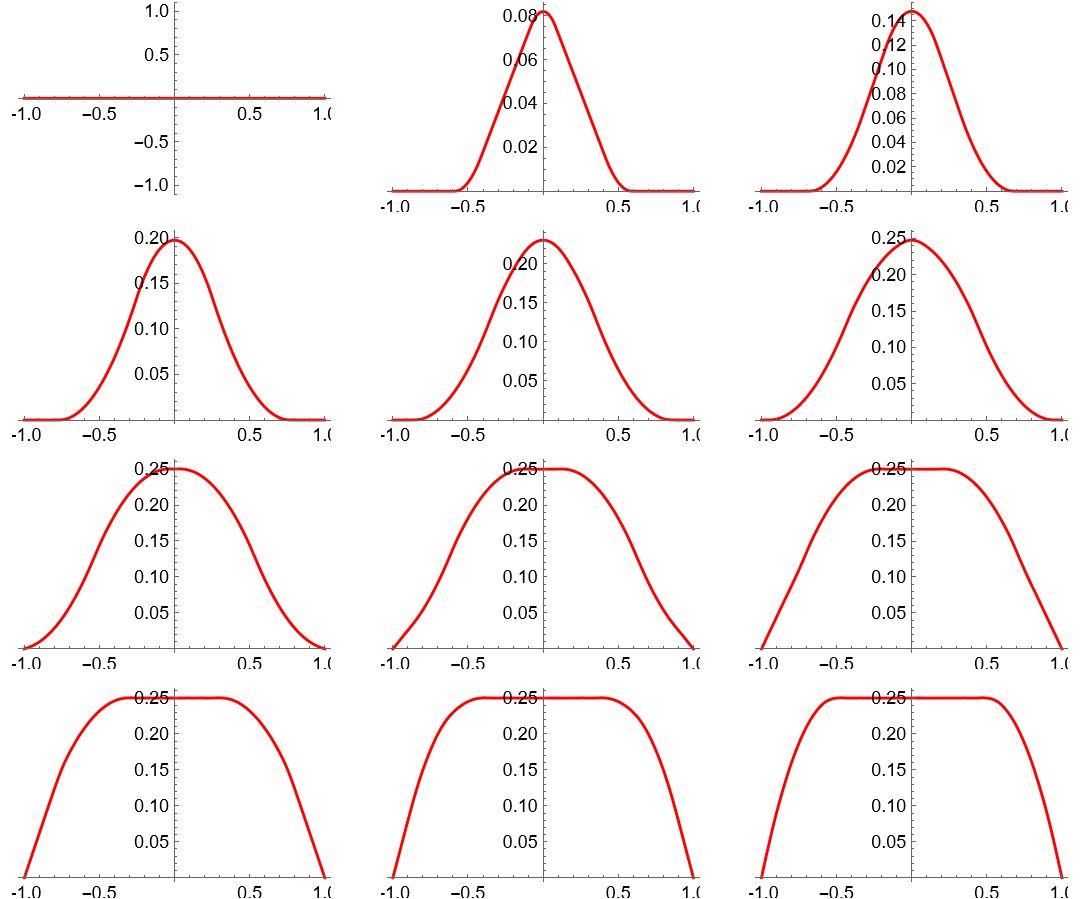
\includegraphics[width=0.7\linewidth]{task2_0.5}
		\caption{Численное решение}
	\end{figure}
	\item $\gamma =0.75\,(\tau = 0.1125 ,h =0.15)$:
	\begin{figure}[H]
		\centering
		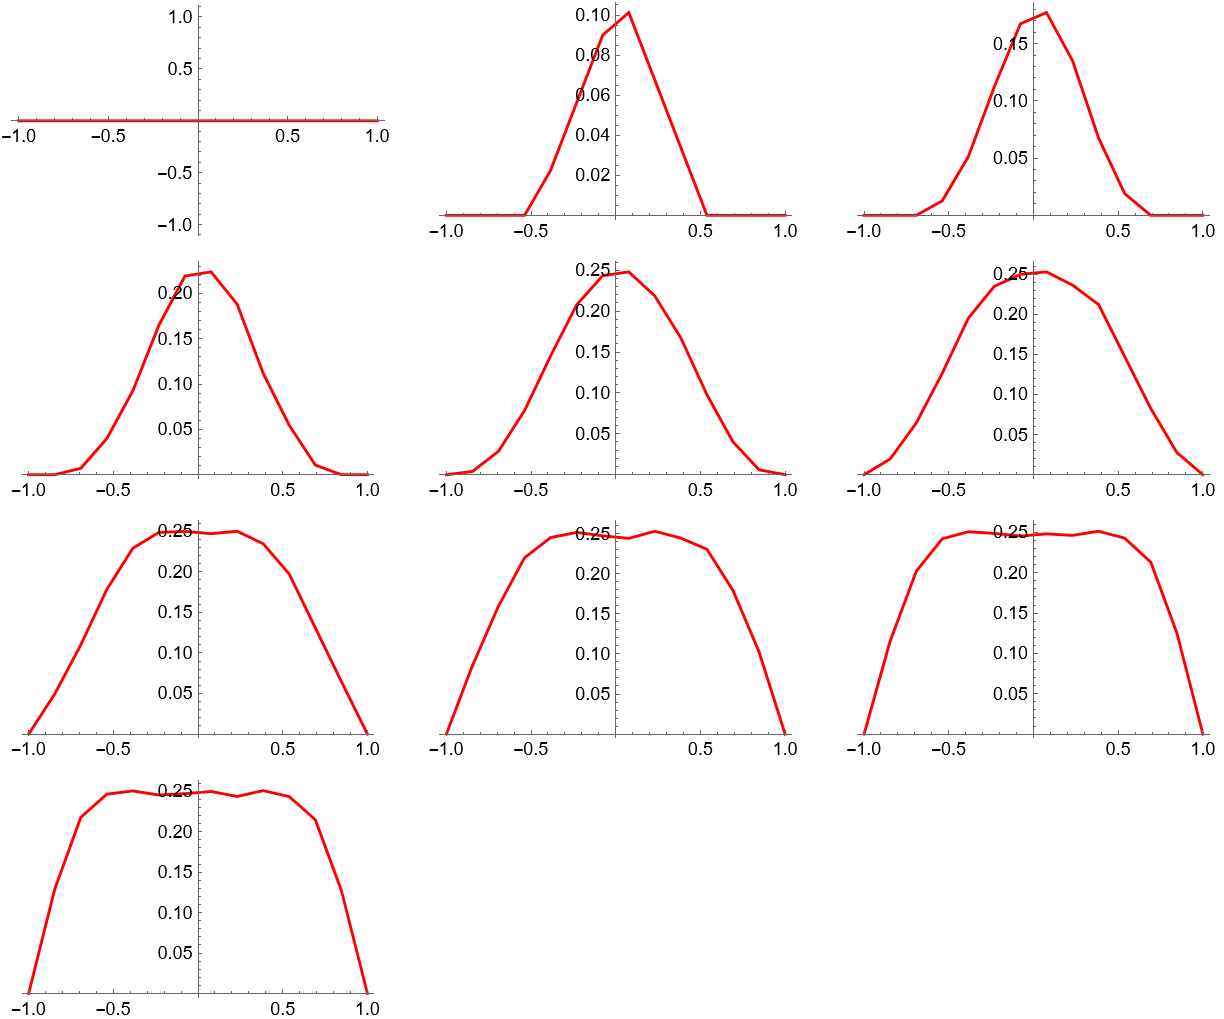
\includegraphics[width=0.7\linewidth]{task2_0.75}
		\caption{Численное решение}
	\end{figure}
\newpage
	\item $\gamma =1.0\,(\tau = 0.01 ,h =0.01)$:
	\begin{figure}[H]
		\centering
		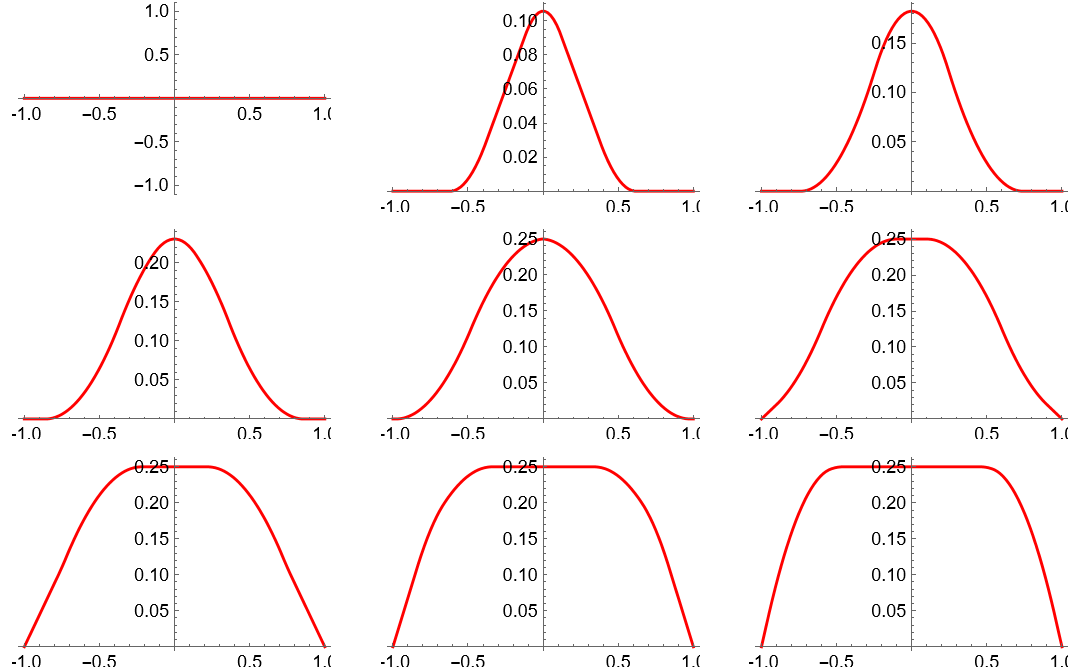
\includegraphics[width=0.7\linewidth]{task2_1.0}
		\caption{Численное решение}
	\end{figure}
\end{enumerate}
\paragraph{Тестовая задача 5}
\[
u_{tt}=u_{xx},\;0<x<4\pi,\;t>0,
\]
\[
u(0,t)=\sin t,\;u(4\pi,t)=0,\;t>0.
\]
\[
u(x,0)=0,\; u_t(x,0)=0,\;0<x<4\pi,
\]
\begin{enumerate}
	\item $\gamma =0.1\,(\tau = 0.01 ,h =0.1)$:
	\begin{figure}[H]
		\centering
		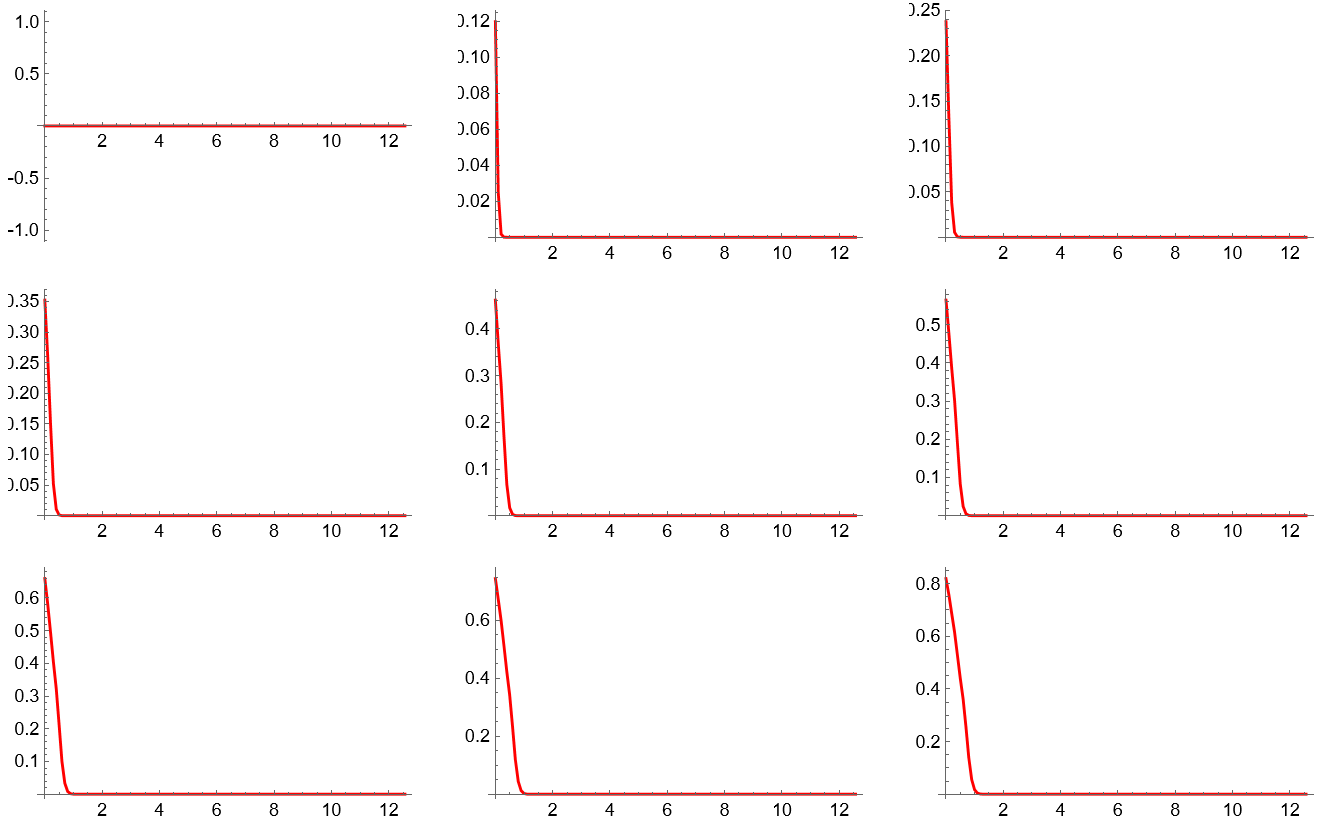
\includegraphics[width=0.7\linewidth]{task3_0.1}
		\caption{Численное решение}
	\end{figure}
\newpage
	\item $\gamma =0.5\,(\tau = 0.01 ,h =0.02)$:
	\begin{figure}[H]
		\centering
		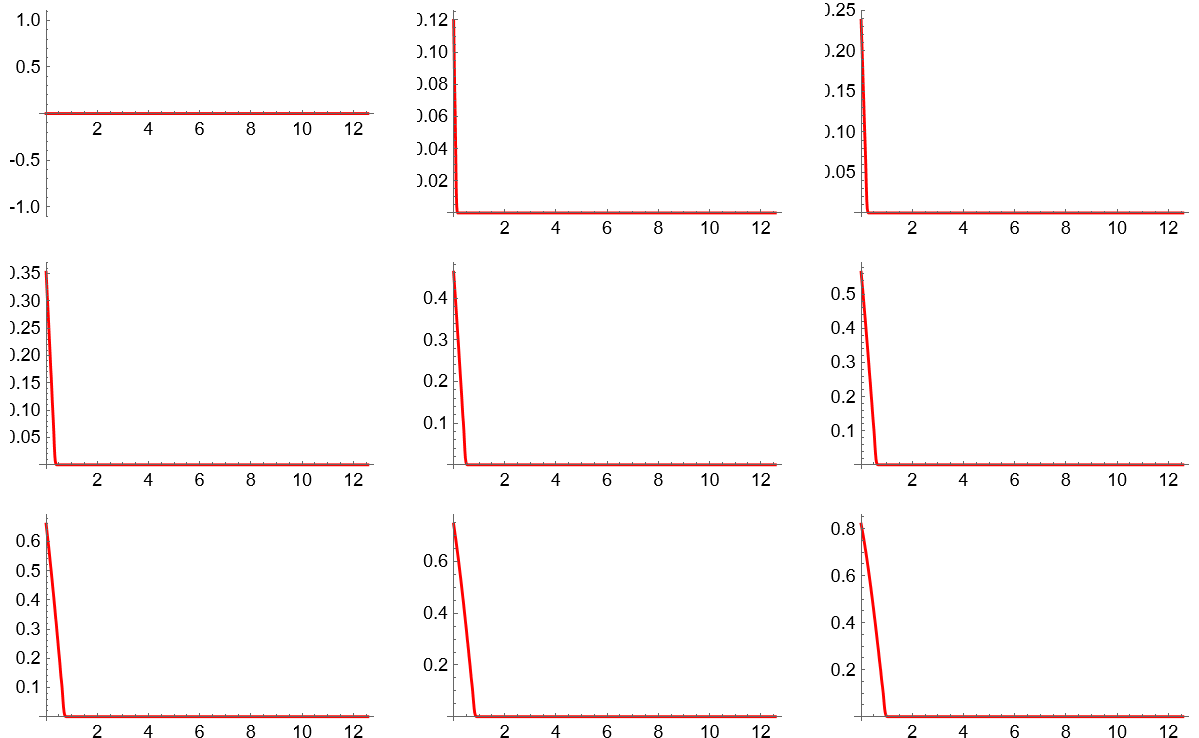
\includegraphics[width=0.7\linewidth]{task3_0.5}
		\caption{Численное решение}
	\end{figure}
	\item $\gamma =0.75\,(\tau = 0.1125 ,h =0.15)$:
	\begin{figure}[H]
		\centering
		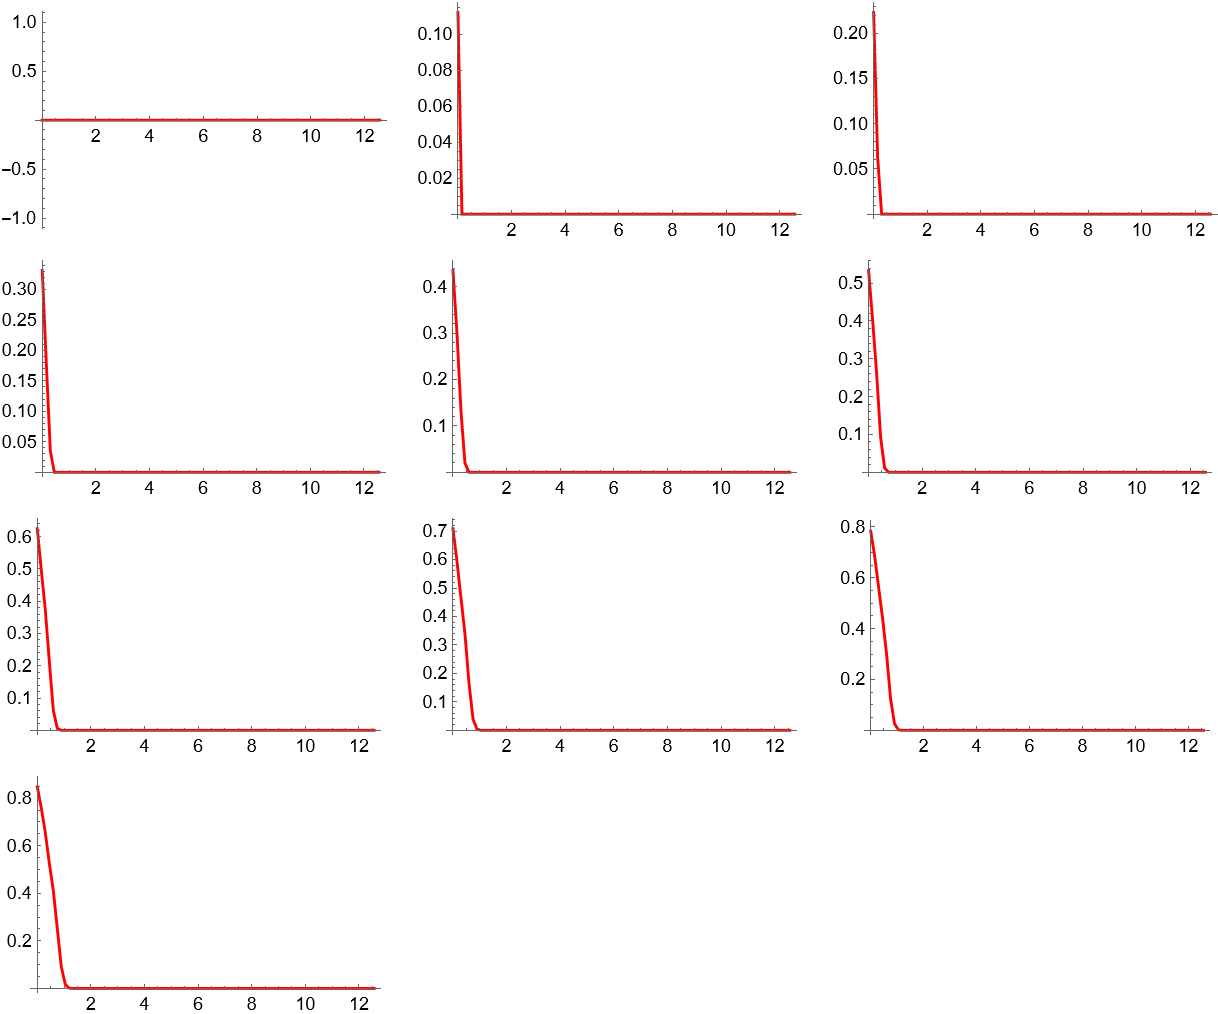
\includegraphics[width=0.7\linewidth]{task3_0.75}
		\caption{Численное решение}
	\end{figure}
\newpage
	\item $\gamma =1.0\,(\tau = 0.01 ,h =0.01)$:
	\begin{figure}[H]
		\centering
		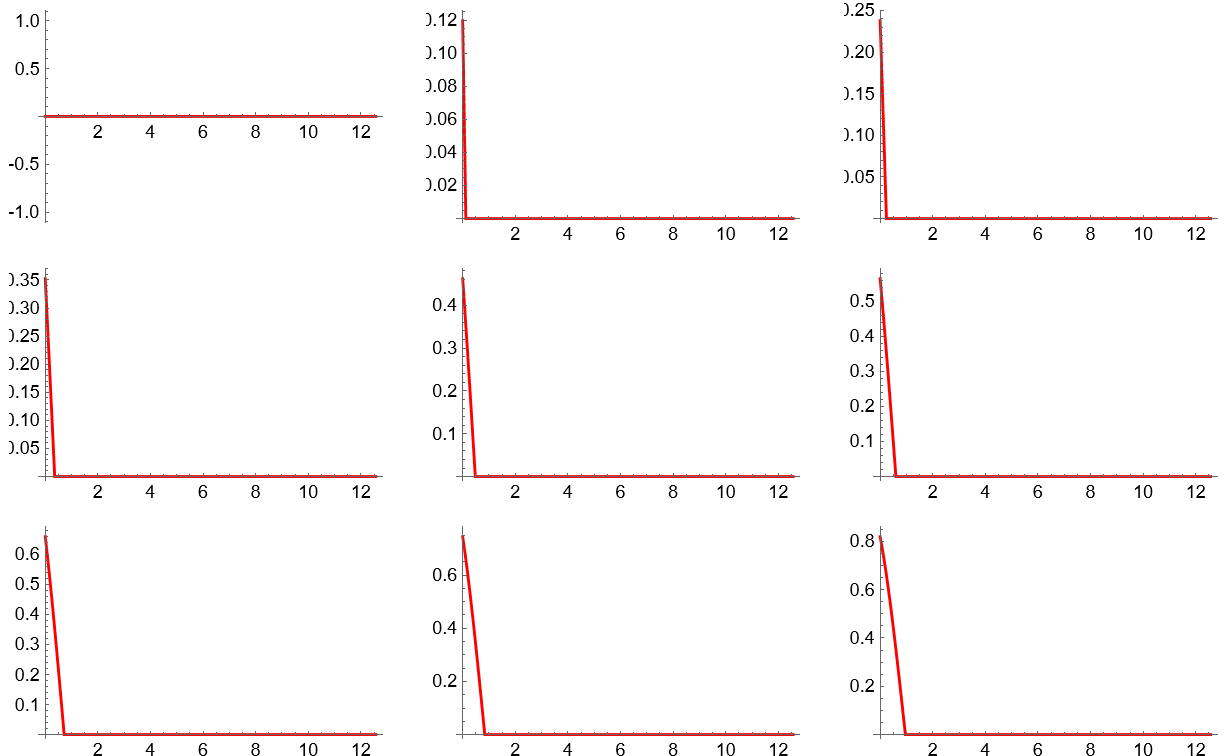
\includegraphics[width=0.7\linewidth]{task3_1.0}
		\caption{Численное решение}
	\end{figure}
\end{enumerate}
\paragraph{Первое дифференциальное приближение}
\[
	u_{tt}=u_{xx},\qquad
	y_{\bar tt}=y_{\bar xx},
	\]
	\begin{multline*}
\psi_h=u_{tt}+\frac{\tau^2}{12}u_{tttt}+O(\tau^4)-u_{xx}-\frac{h^2}{12}u_{xxxx}+O(h^4)=\\=(u_{tt}-u_{xx})+(\frac{\tau^2}{12}u_{tttt}-\frac{h^2}{12}u_{xxxx})+O(\tau^4+h^4).
	\end{multline*} 
\[
u_{tt}=u_{xx},\qquad u_{tttt}=u_{xxtt}=(u_{tt})	_{xx}=u_{xxxx}.
\]
\[
v_{tt}-v_{xx}+\frac{1}{12}(\tau^2-h^2)v_{xxxx}=0,
\]
\[
v_{tt}-v_{xx}+\frac{h^2}{12}(\gamma^2-1)v_{xxxx}=0.
\]
	
	\newpage
	\begin{thebibliography}{1}
		\bibitem{galanin} \textit{Галанин М.П., Савенков Е.Б.} Методы численного анализа математических\\ моделей. М.: Изд-во МГТУ им. Н.Э. Баумана,	2010. 592 с.
		
		
	\end{thebibliography}
	
	
\end{document}
